%!TEX root = ../dissertation.tex

\chapter{Implementation}
\label{implementation}

\section{Flow Overview}

Figure \ref{cha3:methodology:approach} shows the flow of the  the approach taken to deal with determining the orientation of the camera. The coming paragraph gives a brief overview on each of the parts of the procedure, that will be further detailed afterwards.

\begin{figure}[ht]
	\centering
	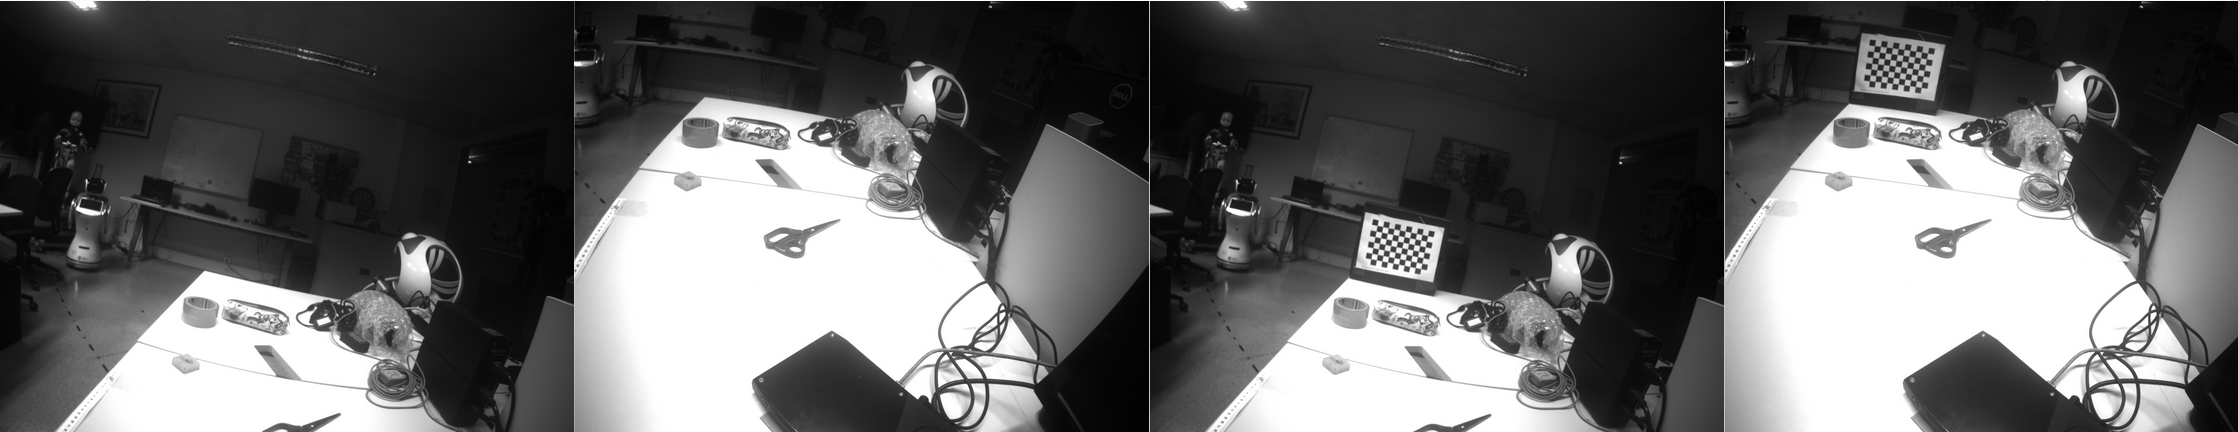
\includegraphics[width=\textwidth]{images/imagesex.png}
	\caption[Example of the two pairs of images]{Example of the two pairs of images. The first and second images are used for finding feature matches and estimating the orientation. The third and fourth images are the same as the first and second ones, respectively, but with a chessboard positioned on the scenery, and serve as ground truth to evaluate the algorithms and the \acrshort{imu}'s performance.}
	\label{cha3:methodology:imagesex}
\end{figure}
	 
\begin{enumerate}
	\item \textbf{Collect images}\\
	Using an uEye LE USB3 camera \footnote{See appendix \ref{appendix:cha2:camera} for camera specifications.}, two grayscale images are collected before and after a certain rotation.
	
	\item \textbf{Collect ground truth}\\
	Using the same camera in the same positions, the two images are taken but positioning a chessboard \footnote{See appendix \ref{appendix:cha2:chessboard} for chessboard specifications.} on the scenery, which is used to determine the ground truth through its regular pattern. The ground truth will then be utilized to evaluate the estimation algorithms performance and also the \acrshort{imu}'s performance over the camera.\\
	
	On Figure \ref{cha3:methodology:imagesex}, an example of the two image pairs that are collected can be observed.
	

	
	\item \textbf{Collect \acrshort{imu}}\\
	The \acrlong{imu} \footnote{See appendix \ref{appendix:cha2:imu} for \acrshort{imu} specifications.} obtains two quaternions (see section \ref{cha2:represent:quat}) with the current camera's orientation before and after rotating.
	
	\item \textbf{Find features and matches}\\
	As stated on section \ref{cha2:features} of the previous chapter,
	\acrshort{sift} and \acrshort{surf} seemed to be the most promising algorithms to detect features on the collected images. Because \acrshort{surf} is faster and more accessible due to patenting concerns regarding \acrshort{sift}, it will be be used on this work.
	\acrshort{flann} also previously referred to in the state of the art will be used for matching the features gathered between the two images, originating a set of point matches. The set of $N$ points matches are pixel coordinates in the first and the second image, $\mathbf{m_{1i}} = [u_{1i} \ v_{1i}]$ and $\mathbf{m_{2i}} = [u_{2i} \ v_{2i}]$, respectively, where $i=1,...,N$.
	
	\item \textbf{Filter outliers}\\
	
\end{enumerate}


\begin{figure}[ht]
	\centering
	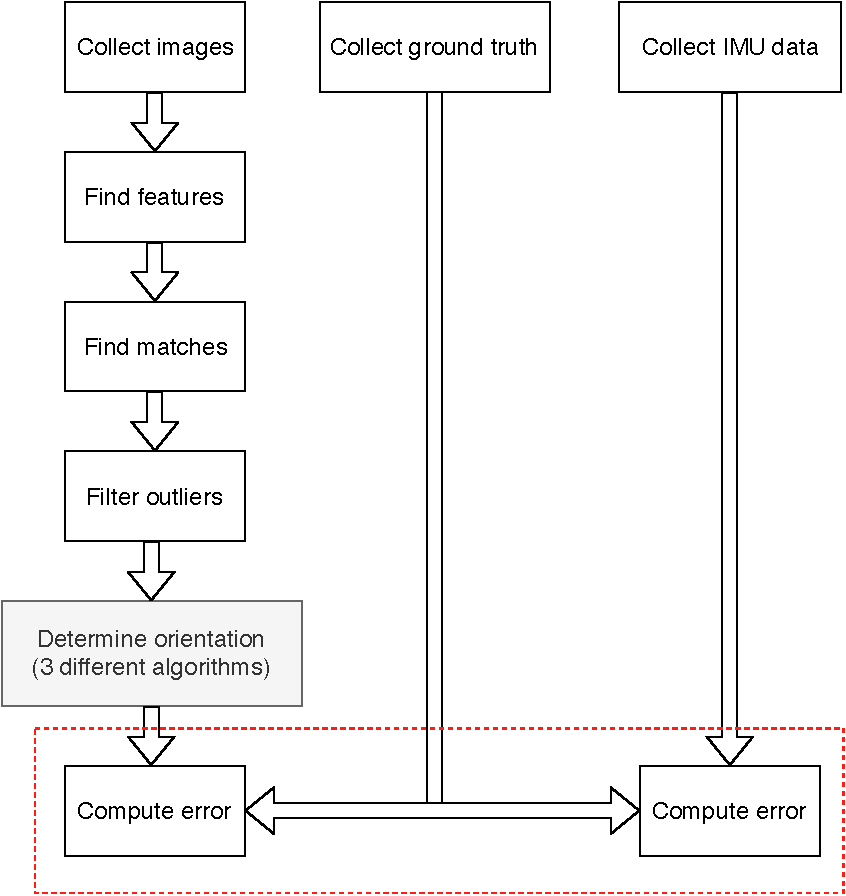
\includegraphics[width=0.7\textwidth]{images/approach.pdf}
	\caption[Approach Diagram]{Approach Diagram. Using the \acrshort{rgb} camera, two images are collected, before and after rotation. In each image, features are detected and matched between them. Some matches might be false or have too much noise, so they are filtered out. Using the matches information, the orientation is determined using an estimation algorithm. 3 algorithms will be put to test. Finally, the orientation determined is compared against the ground truth. The \acrshort{imu}'s orientation output is also compared against the ground truth to evaluate the improvement in relation to the camera.}
	\label{cha3:methodology:approach}
\end{figure}


\subsection{Feature detection and matching}

\subsection{Filtering matches}

\subsection{Simulator}

\subsection{Real world}

\subsubsection{Ground Truth}

Explain how this works on opencv and reference papers. or put on state of the art?

\subsection{C++ Library}



METHOD OF MINIMIZATION LEVEN-MAGEFQ explain what method matlab uses